\documentclass[11pt]{article}

\usepackage{amsmath, amsthm, amssymb}
\usepackage{enumerate}
\usepackage{pdflscape}
\usepackage{caption}
\usepackage{bm}

\usepackage{ifpdf}
\ifpdf
\usepackage[pdftex]{graphicx}
\else
\usepackage[dvips]{graphicx}
\fi
\usepackage{tikz}
 	 \usetikzlibrary{arrows,backgrounds}
\usepackage[all]{xy}

\usepackage{multicol}

\usepackage{tocvsec2}

\usepackage{bbm}

\input xy
\xyoption{all}

\usepackage[pdftex,plainpages=false,hypertexnames=false,pdfpagelabels]{hyperref}
\newcommand{\arxiv}[1]{\href{http://arxiv.org/abs/#1}{\tt arXiv:\nolinkurl{#1}}}
\newcommand{\arXiv}[1]{\href{http://arxiv.org/abs/#1}{\tt arXiv:\nolinkurl{#1}}}
\newcommand{\doi}[1]{\href{http://dx.doi.org/#1}{{\tt DOI:#1}}}
\newcommand{\euclid}[1]{\href{http://projecteuclid.org/getRecord?id=#1}{{\tt #1}}}
\newcommand{\mathscinet}[1]{\href{http://www.ams.org/mathscinet-getitem?mr=#1}{\tt #1}}
\newcommand{\googlebooks}[1]{(preview at \href{http://books.google.com/books?id=#1}{google books})}
\newcommand{\Ws}{\text{W*}}

\usepackage{xcolor}
\definecolor{dark-red}{rgb}{0.7,0.25,0.25}
\definecolor{dark-blue}{rgb}{0.15,0.15,0.55}
\definecolor{medium-blue}{rgb}{0,0,.8}
\definecolor{DarkGreen}{RGB}{0,150,0}
\definecolor{rho}{named}{red}
\hypersetup{
   colorlinks, linkcolor={purple},
   citecolor={medium-blue}, urlcolor={medium-blue}
}

%\addtolength{\textwidth}{.5in}
\usepackage{longtable}
\usepackage{fullpage}
%\renewcommand{\arraystretch}{1.5}

% Page size %%%%%%%%%%%%%%%%%%%%%%%%%%%%%%%%%%%%%%%%%%%
\setlength\topmargin{-.25in}
\setlength\headheight{0in}
\setlength\headsep{.2in}
\setlength\textheight{9in}
%\addtolength{\hoffset}{-0.25in}
%\addtolength{\textwidth}{.5in}
\setlength\parindent{0.25in}

% Theorems %%%%%%%%%%%%%%%%%%%%%%%%%%%%%%%%%%%%%%%%%%
\theoremstyle{plain}
\newtheorem{thm}{Theorem}[]
\newtheorem*{thm*}{Theorem}
\newtheorem{thmalpha}{Theorem}
\renewcommand*{\thethmalpha}{\Alph{thmalpha}}
\newtheorem{cor}[thm]{Corollary}
\newtheorem{coralpha}[thmalpha]{Corollary}
\newtheorem*{cor*}{Corollary}
\newtheorem{conj}[thm]{Conjecture}
\newtheorem{conjalpha}[thmalpha]{Conjecture}
\newtheorem*{conj*}{Conjecture}
\newtheorem{lem}[thm]{Lemma}
\newtheorem{fact}[thm]{Fact}
\newtheorem{facts}[thm]{Facts}
\newtheorem{prop}[thm]{Proposition}
\newtheorem{quest}[thm]{Question}
\newtheorem*{quest*}{Question}
\newtheorem*{claim*}{Claim}
\newtheorem{quests}[thm]{Questions}
\theoremstyle{definition}
\newtheorem{defn}[thm]{Definition}
\newtheorem{construction}[thm]{Construction}
\newtheorem{alg}[thm]{Algorithm}
\newtheorem{assumption}[thm]{Assumption}
\newtheorem{nota}[thm]{Notation}
\newtheorem{nb}[thm]{Note}
\newtheorem{note}[thm]{Note}
\newtheorem{exs}[thm]{Examples}
\newtheorem{ex}[thm]{Example}
\newtheorem{exercise}[thm]{Exercise}
\newtheorem{sub-ex}[thm]{Sub-Example}
\newtheorem{rem}[thm]{Remark}
\newtheorem*{rem*}{Remark}
\newtheorem{remark}[thm]{Remark}
\newtheorem{rems}[thm]{Remarks}
\newtheorem{warn}[thm]{Warning}

% Operators %%%%%%%%%%%%%%%%%%%%%%%%%%%%%%%%%%%%%%%%%%%
\DeclareMathOperator{\Ad}{Ad}
\DeclareMathOperator{\Aut}{Aut}
\DeclareMathOperator{\coev}{coev}
\DeclareMathOperator{\Dom}{Dom}
\DeclareMathOperator{\End}{End}
\DeclareMathOperator{\ev}{ev}
\DeclareMathOperator{\Hom}{Hom}
\DeclareMathOperator{\Mor}{Mor}
\DeclareMathOperator{\op}{op}
\DeclareMathOperator{\ONB}{ONB}
\DeclareMathOperator{\Ob}{Ob}
\DeclareMathOperator{\rev}{rev}
\DeclareMathOperator{\spann}{span}
\DeclareMathOperator{\supp}{supp}
\DeclareMathOperator{\id}{id}
\DeclareMathOperator{\Isom}{Isom}
\DeclareMathOperator{\ind}{ind}
\DeclareMathOperator{\im}{im}
\DeclareMathOperator{\Irr}{Irr}
\DeclareMathOperator{\Spec}{Spec}
\DeclareMathOperator{\Stab}{Stab}
\DeclareMathOperator{\Tr}{Tr}
\DeclareMathOperator{\tr}{tr}
\DeclareMathOperator{\Gr}{Gr}


% Math %%%%%%%%%%%%%%%%%%%%%%%%%%%%%%%%%%%%%%%%%%%%%
\newcommand{\D}{\displaystyle}
\newcommand{\comment}[1]{}
\newcommand{\hs}{\hspace{.07in}}
\newcommand{\hsp}[1]{\hs\text{#1}\hs}
\newcommand{\be}{\begin{enumerate}[label=(\arabic*)]}
\newcommand{\ee}{\end{enumerate}}
\newcommand{\itm}[1]{\item[\underline{\ensuremath{#1}:}]}
\newcommand{\itt}[1]{\item[\underline{\text{#1}:}]}
\newcommand{\N}{\mathbb{N}}
\newcommand{\Natural}{\mathbb{N}}
\newcommand{\Z}{\mathbb{Z}}
\newcommand{\Q}{\mathbb{Q}}
\newcommand{\F}{\mathbb{F}}
\newcommand{\R}{\mathbb{R}}
\newcommand{\C}{\mathbb{C}}
\newcommand{\B}{\mathbb{B}}
\renewcommand{\P}{\mathbb{P}}
\newcommand{\I}{\infty}
\newcommand{\set}[2]{\left\{#1 \middle| #2\right\}}
\newcommand{\thh}{^{\text{th}}}
\renewcommand{\a}{\mathfrak{a}}
\renewcommand{\b}{\mathfrak{b}}
\renewcommand{\c}{\mathfrak{c}}
\newcommand{\n}{\mathfrak{n}}
\newcommand{\m}{\mathfrak{m}}
\newcommand{\bbOne}{\mathbbm{1}}
\renewcommand{\alg}[1]{{\bm{\langle} #1\bm{\rangle}}}


% some math commands specific to this document %%%%%%%%%%%%
\newcommand{\xalt}{x^{\text{alt}\otimes n}}
\newcommand{\xbaralt}{\overline{x}^{\text{alt}\otimes n}}
%%%%%%%%%%%%%%%%%%%%%%%%%%%%

\newcommand{\dave}[1]{\marginpar{\tiny \textcolor{orange}{DP: #1}}}
\newcommand{\corey}[1]{\marginpar{\tiny \textcolor{green}{CJ: #1}}}
\newcommand{\Af}{\mathcal{A}\Lambda_{F}}
\newcommand{\WStar}{\bfW\text{*}}
%\newcommand{\Irr}{\text{Irr}(\mathcal{C})}

% tricky way to iterate macros over a list
\def\semicolon{;}
\def\applytolist#1{
    \expandafter\def\csname multi#1\endcsname##1{
        \def\multiack{##1}\ifx\multiack\semicolon
            \def\next{\relax}
        \else
            \csname #1\endcsname{##1}
            \def\next{\csname multi#1\endcsname}
        \fi
        \next}
    \csname multi#1\endcsname}

% \def\cA{{\cal A}} for A..Z
\def\calc#1{\expandafter\def\csname c#1\endcsname{{\mathcal #1}}}
\applytolist{calc}QWERTYUIOPLKJHGFDSAZXCVBNM;
% \def\bbA{{\mathbb A}} for A..Z
\def\bbc#1{\expandafter\def\csname bb#1\endcsname{{\mathbb #1}}}
\applytolist{bbc}QWERTYUIOPLKJHGFDSAZXCVBNM;
% \def\bfA{{\mathbf A}} for A..Z
\def\bfc#1{\expandafter\def\csname bf#1\endcsname{{\mathbf #1}}}
\applytolist{bfc}QWERTYUIOPLKJHGFDSAZXCVBNM;
% \def\sA{{\sf A}} for A..Z
\def\sfc#1{\expandafter\def\csname s#1\endcsname{{\sf #1}}}
\applytolist{sfc}QWERTYUIOPLKJHGFDSAZXCVBNM;
% \def\fA{{\mathfrak A}} for A..Z
\def\fc#1{\expandafter\def\csname f#1\endcsname{{\mathfrak #1}}}
\applytolist{fc}QWERTYUIOPLKJHGFDSAZXCVBNM;


\newcommand{\PA}{\cP\hspace{-.1cm}\cA}
\newcommand{\Fun}{{\sf Fun}}
\newcommand{\Rep}{{\sf Rep}}
\newcommand{\Set}{{\sf Set}}
\newcommand{\FreeMod}{{\sf FreeMod}}
\newcommand{\Mod}{{\sf Mod}}
\newcommand{\Proj}{{\sf Proj}}
\newcommand{\AlgBim}{{\sf AlgBim}}
\newcommand{\Bim}{{\sf Bim}}
\newcommand{\bfBim}{{\sf Bim_{bf}}}
\newcommand{\spBim}{{\sf Bim^{sp}}}
\newcommand{\spbfBim}{{\sf Bim_{bf}^{sp}}}
\renewcommand{\Vec}{{\sf Vec}}
\newcommand{\fdVec}{{\sf Vec_{fd}}}
\newcommand{\Hilb}{{\sf Hilb}}
\newcommand{\fdHilb}{{\sf Hilb_{fd}}}
\newcommand{\ConAlg}{{\sf ConAlg}}
\newcommand{\DisInc}{{\sf DisInc}}


\newcommand{\jw}[1]{f^{(#1)}}
\newcommand{\todo}[1]{\textcolor{blue}{\textbf{TODO: #1}}}
\newcommand{\nn}[1]{\textcolor{red}{[[#1]]}}
\newcommand{\noshow}[1]{}
\newcommand{\MR}[1]{}
\newcommand{\TL}{\cT\hspace{-.08cm}\cL}
\newcommand{\rhoE}{\textcolor{rho}{e_1}}
\newcommand{\rhoJW}{\textcolor{rho}{\jw{2}}}


% TikZ operators %%%%%%%%%%%%%%%%%%%%%%%%%%%%%%%%%%%%%%%%
\usetikzlibrary{shapes}
\usetikzlibrary{cd}
\usetikzlibrary{backgrounds}
\usetikzlibrary{decorations,decorations.pathreplacing,decorations.markings}
\usetikzlibrary{fit,calc,through}
\usetikzlibrary{external}
\usetikzlibrary{arrows}
\tikzset{vertex/.style = {shape=circle,draw,fill=black,inner sep=0pt,minimum size=5pt}}
\tikzset{edge/.style = {->,> = latex', bend right}}
\tikzset{
	super thick/.style={line width=3pt}
}
\tikzset{
    quadruple/.style args={[#1] in [#2] in [#3] in [#4]}{
        #1,preaction={preaction={preaction={draw,#4},draw,#3}, draw,#2}
    }
}
\tikzstyle{shaded}=[fill=red!10!blue!20!gray!30!white]
\tikzstyle{unshaded}=[fill=white]
\tikzstyle{empty box}=[circle, draw, thick, fill=white, opaque, inner sep=2mm]
\tikzstyle{annular}=[scale=.7, inner sep=1mm, baseline]
\tikzstyle{rectangular}=[scale=.75, inner sep=1mm, baseline=-.1cm]
\tikzstyle{mid>}=[decoration={markings, mark=at position 0.5 with {\arrow{>}}}, postaction={decorate}]
\tikzstyle{mid<}=[decoration={markings, mark=at position 0.5 with {\arrow{<}}}, postaction={decorate}]
\tikzstyle{over}=[double, draw=white, super thick, double=]

\newcommand{\roundNbox}[6]{
	\draw[rounded corners=5pt, very thick, #1] ($#2+(-#3,-#3)+(-#4,0)$) rectangle ($#2+(#3,#3)+(#5,0)$);
	\coordinate (ZZa) at ($#2+(-#4,0)$);
	\coordinate (ZZb) at ($#2+(#5,0)$);
	\node at ($1/2*(ZZa)+1/2*(ZZb)$) {#6};
}


\newcommand{\nbox}[6]{
	\draw[thick, #1] ($#2+(-#3,-#3)+(-#4,0)$) rectangle ($#2+(#3,#3)+(#5,0)$);
	\coordinate (ZZa) at ($#2+(-#4,0)$);
	\coordinate (ZZb) at ($#2+(#5,0)$);
	\node at ($1/2*(ZZa)+1/2*(ZZb)$) {#6};
}

\newcommand{\ncircle}[4]{
	\draw[very thick, #1] #2 circle (#3);
	\node at #2 {#4};
%	\filldraw[red] ($#2+(#4:#3cm)$) circle (.05cm);
%	\node at ($#2+(#4:.15cm)+(#4:#3cm)$) {$\star$};
}

  \newcommand{\tikzmath}[2][]
     {\vcenter{\hbox{\begin{tikzpicture}[#1]#2
                     \end{tikzpicture}}}
     }

% colors %%%%%%%%%%%%%%%%%%%%%%%%%%%%%%%%%%%%%%%%
\newcommand{\cupcolor}{DarkGreen}
\newcommand{\alphacolor}{blue}
\newcommand{\betacolor}{red}

% title %%%%%%%%%%%%%%%%%%%%%%%%%%%%%%%%%%%%%%%%%

\title{The Embedding Theorem for Module Categories}
\author{Desmond Coles, Peter Huston, David Penneys, \& Srivatsa Srinivas}





%%%%%%%%%%%%%%%%%%%%%%%%%%%%%%%%%%%%%%


\usepackage[utf8]{inputenc}
\begin{document}


%%%%%%%%%%%%%%%%%%%%%%%%%%%%%%%%%%%%%%%%%%%%%%%%%%%%%%%%%%%%%%%
%%%%%%%%%%%%%%%%%%%%%%%%%%%%%%%%%%%%%%%%%%%%%%%%%%%%%%%%%%%%%%%
%%%%%%%%%%%%%%%%%%%%%%%%%%%%%%%%%%%%%%%%%%%%%%%%%%

\maketitle
\begin{abstract}
Please read our paper it's great, like really really great seriously please.
\end{abstract}
\section{Introduction}
\section{Preliminaries}
\section{Construction of the Planar Algebra Associated to a Module Category}
\subsection{Construction of a Markov Sequence}
Given a subfactor planar algebra $Q_{\bullet}$, let $\cC$ be the paragroup of $Q_{\bullet}$ and $\cM$ be an indecomposable module category for $\cC$. We know that there is a $3\times 3$ unitary multifusion category $\widetilde{\cC}$, with $1_{\widetilde{\cC}}= 1_0 \oplus 1_1 \oplus 1_2$ and $\cC$ the  non-unital $2\times 2$ unitary multifusion subcategory with $1_\cC = 1_0\oplus 1_1$, so that $\cM\cong\cC_{20}\oplus \cC_{21}$. Overall,
$$
\cM 
=
\begin{pmatrix}
\cC_{20} & \cC_{21} 
\end{pmatrix}
\qquad\qquad
\cC
=
\begin{pmatrix}
\cC_{00} & \cC_{01} 
\\
\cC_{10} & \cC_{11}
\end{pmatrix}
\subset
\begin{pmatrix}
\cC_{00} & \cC_{01} & \cC_{02}
\\
\cC_{10} & \cC_{11} & \cC_{12}
\\
\cC_{20} & \cC_{21} & \cC_{22}
\end{pmatrix}
=
\widetilde{\cC}
$$

Let $x\in \cC_{01}$ be the strand pictured below:

$$x=

\begin{tikzpicture}[baseline=-.1cm]
	\fill[white] (0,-.7) rectangle (-.7,-.7);
	\fill[gray!25!white] (0,-.7) rectangle (.7,.7);
	\draw (0,-.7) -- (0,.7);

\end{tikzpicture}
\ \,\,\,\,\, \text{and,}\,\,\,\,\, \overline{x}=

\begin{tikzpicture}[baseline=-.1cm]
	\fill[white] (0,-.7) rectangle (.7,.7);
	\fill[gray!25!white] (0,-.7) rectangle (-.7,.7);
	\draw[fill] (0,-.7) -- (0,.7);

\end{tikzpicture}
\,\,\,\,\, \text{so} \,\,\,\,\, x\otimes \overline{x} = 
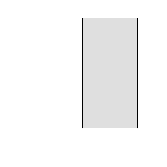
\begin{tikzpicture}[baseline=-.1cm]
	\fill[white] (0,-.7) rectangle (-.7,.7);
	\fill[gray!25!white] (0,-.7) rectangle (.7,.7);
	\draw (0,-.7) -- (0,.7);
	\draw (.7,-.7) -- (.7,.7);

\end{tikzpicture}
$$

By construction, $x$ is a generating object for $\cC$. If we pick a simple object $m\in \cC_{20}$, since $\cM$ is indecomposable, we have that any object of $\cM$ is isomorphic to a direct summand of $m\otimes \xalt$ for some nonnegative integer $n$, where $$
x^{\text{alt}\otimes n}:=\underbrace{x\otimes \overline{x} \otimes x \otimes \cdots \otimes x^?}_{n \text{ tensorands}}\,,
$$ and $x^? = \overline x$ if $n$ is even and $x$ if $n$ is odd. We define $\xbaralt$ similarly.

We will construct a finite depth Markov sequence of algebras from the action of $\cC$ on $\cM$ as follows. Set $A_n=\End_{\cC}(m\otimes \xalt)$. We can represent morphisms in $A_n$ as 
$$
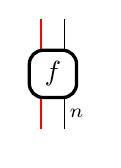
\begin{tikzpicture}[baseline=.4cm]
	\draw[thick, red] (-.15,-.7) -- (-.15,.7);
	\draw (.15,-.7) -- (.15,.7);
	
	\roundNbox{unshaded}{(0,0)}{.3}{0}{0}{$f$}
	
	\node at (.3,-.5) {\scriptsize{$n$}};

\end{tikzpicture}
$$
where the red strand represents $m$ and the $n$ represents $x^{\text{alt}\otimes n}$. We have a faithful tracial state $\tr_n:A_n\to \C$ given by
\begin{equation}\label{eq:TraceAn}
\tr_n(f) 
\,:=\, 
\frac{1}{\dim_\cC(m)\dim_\cC(x)^n}\cdot\tr_\cC(f)
\,=\,
\frac{1}{\dim_\cC(m)}\cdot
\frac{1}{d^n}
\cdot
\left(
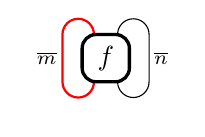
\begin{tikzpicture}[baseline=-.1cm, rotate=90]
	\draw[thick, red] (-.3,.15) arc (270:90:.2cm) -- (.3,.55) arc (90:-90:.2cm);
	\draw (-.3,-.15) arc (90:270:.2cm) -- (.3,-.55) arc (-90:90:.2cm);
	\roundNbox{unshaded}{(0,0)}{.3}{0}{0}{$f$}
%	\node at (-.7,-.35) {\scriptsize{$n$}};
	\node at (0,-.7) {\scriptsize{$\overline{n}$}};
	\node at (0,.75) {\scriptsize{$\overline{m}$}};
%	\node at (.7,.35) {\scriptsize{$m$}};
\end{tikzpicture}
\right)
\end{equation}
Where $n$ and $\overline{n}$ represent $\xalt$ and $\xbaralt$, respectively. This makes each $A_n$ a finite dimensional von Neumann algebra.

\begin{rem}
	The trace can be identified with a complex scalar because $\overline{m}\otimes m\in\cC_{00}$, the red cup $1\to\overline{m}\otimes m$ and cap $\overline{m}\otimes m\to 1$ factor through the simple summand $1_0$. Since $1_0\otimes 1\cong 1_0$, the trace is a member of the $1$-dimensional algebra $\End(1_0)\subseteq\End(1)$. 
\end{rem}

We also have a natural tracial inclusion $A_n \rightarrow A_{n+1}$. % such that the trace restricts ($tr_{n+1}|_{A_n}=tr_n$):
\begin{equation}\label{eq:Inclusion}
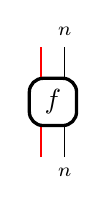
\begin{tikzpicture}[baseline=-.1cm, rotate=90]
	\draw[thick, red] (-.7,.15) -- (.7,.15);
	\draw (-.7,-.15) -- (.7,-.15);
	\roundNbox{unshaded}{(0,0)}{.3}{0}{0}{$f$}
	\node at (-.9,-.15) {\scriptsize{$n$}};
	\node at (.9,-.15) {\scriptsize{$n$}};
\end{tikzpicture}
\mapsto
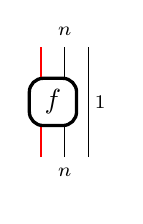
\begin{tikzpicture}[baseline=-.2cm, rotate=90]
	\draw[thick, red] (-.7,.15) -- (.7,.15);
	\draw (-.7,-.15) -- (.7,-.15);
	\draw (-.7,-.45) -- (.7,-.45);
	\roundNbox{unshaded}{(0,0)}{.3}{0}{0}{$f$}
	\node at (-.9,-.15) {\scriptsize{$n$}};
	\node at (.9,-.15) {\scriptsize{$n$}};
	\node at (0,-.6) {\scriptsize{$1$}};
\end{tikzpicture}
\end{equation}

and a trace preserving conditional expectation $E_n:A_n\rightarrow A_{n-1}$, left inverse to the inclusion

\begin{equation}\label{eq:ConditionalExpectationAn}
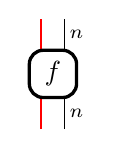
\begin{tikzpicture}[baseline=-.1cm]
	\draw[thick, red] (-.15,-.7) -- (-.15,.7);
	\draw (.15,-.7) -- (.15,.7);
	\roundNbox{unshaded}{(0,0)}{.3}{0}{0}{$f$}
	\node at (.3,.5) {\scriptsize{$n$}};
	\node at (.3,-.5) {\scriptsize{$n$}};
\end{tikzpicture}
\mapsto\,
\frac{1}{d}
\cdot
\left(\,\,
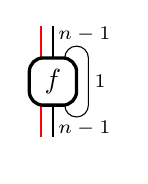
\begin{tikzpicture}[baseline=-.1cm]
	\draw[thick, red] (-.15,-.7) -- (-.15,.7);
	\draw (0,-.7) -- (0,.7);
	\draw (.15,.3) arc (180:0:.15cm) -- (.45,-.3) arc (0:-180:.15cm);
	\roundNbox{unshaded}{(0,0)}{.3}{0}{0}{$f$}
	\node at (.4,.6) {\scriptsize{$n-1$}};
	\node at (.4,-.6) {\scriptsize{$n-1$}};
	\node at (.6,0) {\scriptsize{$1$}};
\end{tikzpicture}
\right)
\end{equation}

Here, $d:=\dim_{\cC}(x)=\dim_{\cC}(\overline{x})$ the value of a closed loop appearing in the diagram. % There must be a better word for this. Maybe we should also remark why these are equal? In response: Emily peter's uses the term closed circles (on page 7 of her thesis), if that's the woridng you mean, and the equality follows from sphericality, maybe we should this should probably be in the preliminary discussion of the paragroup and the constructed multifusion category
Given the previously defined inclusion and that multiplication is given by vertical stacking of diagrams, it's clear that $E_n$ is $A_{n-1}$ bilinear. Similarly, we have that $tr_n=tr_{n-1} \circ E_n$.

Finally, the Jones projections for each inclusion $A_{n}\subset A_{n+1}$ are given by

\begin{equation}\label{eq:JonesProjections}
e_n=
\frac1d\cdot
\left(\,\,
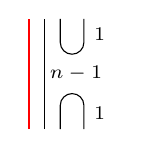
\begin{tikzpicture}[baseline=-.1cm]
	\draw[thick, red] (-.3,-.7) -- (-.3,.7);
	\draw (-.1,-.7) -- (-.1,.7);
	\draw (.1,-.7) -- (.1,-.4) arc (180:0:.15cm) -- (.4,-.7);
	\draw (.1,.7) -- (.1,.4) arc (-180:0:.15cm) -- (.4,.7);
%	\node at (-.1,-1) {\scriptsize{$n-1$}};
	\node at (.3,0) {\scriptsize{$n-1$}};
	\node at (.6,.5) {\scriptsize{$1$}};
	\node at (.6,-.5) {\scriptsize{$1$}};
\end{tikzpicture}
\right)
\in
A_{n+1}.
\end{equation}

Where the $n-1$ indicates $n-1$ vertical strands with appropriate shading to the right of the red strand. The Temperley-Lieb- % strange editor enforced wordwrap from here. lint?
Jones relations follow immediately from the definition and the fact that closed loops count for a factor of $d$. Similarly, 
for any $x\in A_n$ we have $e_nxe_n=E_n(x)e_n$. Clearly, $E_{n+1}(e_n)=d^{-2}id_{m \otimes \xalt}$. Finally, the pull 
down condition % probably we should define the condition somewhere in the prelims, and then this becomes ``(some number)''; if not, then we should explicitly give the condition here, whatever it is. 
holds, as for each $x\in A_{n+1}$, we have that $d^2 E_{n+1}(xe_n)e_n=xe_n$. Equivalently, $A_{n} e_n A_n$ is a 
two-sided ideal in $A_{n+1}$. Thus, the tower algebras given by the $A_n$ is indeed a Markov sequence.
 
\begin{prop}
The Markov sequence of von Neumann Algebras $(A_n, tr_n)_{n\geq 0}$ is finite depth.
\end{prop}

\begin{proof}
$m\otimes \xalt$ generates $\cM$. Let $s^i_1,\ldots s^i_{r_i}$, for $i=0$ or $1$ be a collection of non-isomorphic simple objects spanning $\cC_{2i}$. Recall that $\Hom_{\cC}(s^i_k,s^i_l)\cong \delta_{kl}\bbC$, 

% warning: a lot of indices are undefined and text is missing in this block. 
$$\End_{\cC}(m\otimes\xalt)\cong \bigoplus\limits_{j}\End_{\cC}(n_j s^i_j) \cong \bigoplus\limits_{j}M_{n_j}(\bbC)$$
If we have that 
$$m \otimes \xalt \cong \bigoplus\limits_{j}n_js^i_j$$
	where $i=n\text{ mod }2$, then 
$$n_js^i_j:=\underbrace{s^i_j\oplus s^i_j\oplus \cdots \oplus s^i_j}_{n_j \,\, \text{summands}}$$

Thus, at each level of the Bratteli diagram corresponding to $A_n$ % should be an inclusion, 
	there are at most $\max\{r_1,r_0\}$ vertices, so the principal graph must be finite. % remark that the principal graph is (contained in?) the direct limit of Bratteli diagrams or something? Unclear what this implies in the infinite case... In reponse: the veritce correspond to the algebras, edges to these inclusions which is why I worded it the way I did.
\end{proof}

\begin{thm}
The principal graph obtained from the Markov sequence $(A_n)_{n\geq 0}$ is independent of the choice of $m$, and is in fact isomorphic to the fusion graph for $\cM$.
\end{thm}

\begin{proof}
First, recall that for a finite depth Markov sequence, the principal graph is canonically isomorphic to the Bratteli for the inclusion $A_n\subset A_{n+1}$ for $n$ large enough that this inclusion is standard. So, it suffices to show this Bratteli diagram is isomorphic to the fusion graph for $\cM$. 

Let $s^i_1,\ldots s^i_{r_i}$, for $i=0$ or $1$ be a collection of non-isomorphic simple objects in $\cC_{2i}$ such that every object in $\cC_{2i}$ is isomorphic to a direct sum of these elements, as in the previous proof. 
	We will work the index $i$ mod 1 so that we may write $s^{i+1}_j$ for brevity of notation. % no idea what this can mean
	Let the non-negative integers $p^{i,j}_k$ be defined by the following equation:

$$s^i_j\otimes x^{?}=\bigoplus\limits_{k=1}^{r_{i+1}}p^{i,j}_ks^{i+1}_k$$

where $x^{?}$ is $x$ if $n$ is even and $\overline{x}$ if $n$ is odd. % This is dual to the previous definition of x^?. But I don't understand what is going on so I can't tell if it is correct. 
	These coefficients are exactly the coefficients for the adjacency matrix of the fusion graph for $x^{?}$.

Recall from the previous proof that:

$$A_n=\End_{\cC}(m\otimes\xalt)\cong \bigoplus\limits_{j}\End_{\cC}(n_j s^i_j) \cong \bigoplus\limits_{j}M_{n_j}(\bbC)$$
if we have that 
$$m \otimes \xalt \cong \bigoplus\limits_{j}n_js^i_j$$
Note that we may take $n$ such that all $n_j$ are strictly positive, as there is some $n$ such that $s^{i}_1\oplus\cdots \oplus s^{i}_{r_i}$ is isomorphic to a direct summand of $m\otimes \xalt$ (in fact the first $n$ where this happens is exactly when the Markov sequence achieves depth). But now, we know that:

$$A_{n+1}=\End_{\cC}(m\otimes\xalt\otimes x^{?})\cong \bigoplus\limits_{k=1}^{r_{i+1}}\End_{\cC}(\sum\limits_{j=1}^{r_i}(p^{i,j}_kn_j)s^{i+1}_k)\cong M_{(\sum\limits_{j=1}^{r_i}p^{i,j}_k n_j)}(\bbC)$$

Furthermore, the inclusion of $A_n \hookrightarrow A_{n+1}$ is a unital inclusion, given by $\phi \mapsto \phi \otimes \id_{x^{?}}$. Each $\phi \in A_n$ is uniquely defined as a direct sum 
$$\bigoplus\limits_{j=1}^{r_i}\phi_j$$
where each $\phi_j$ is an element of $\End_{\cC}(n_js^{i}_j)$. Then, distributing tensor products over the sum, we may write $\phi$ as 
$$\bigoplus_{j=1}^{r_i}(\phi_j \otimes \id_{x^{?}})$$
But then:
$$\phi_j \otimes \id_{x^{?}}\in \End_{\cC}(n_js^{i}_j\otimes x^{?})\cong \End_{\cC}(\bigoplus\limits_{k=1}^{r_{i+1}}n_jp^{i,j}_ks^{i+1}_k)\cong \bigoplus\limits_{k=1}^{r_{i+1}}\End_{\cC}(n_jp^{i,j}_ks^{i+1}_k)\cong \bigoplus\limits_{k=1}^{r_{i+1}}M_{(n_jp^{i,j}_k)}(\bbC)$$

Since all $n_j\neq 0$, we have that the $j$th summand of $A_n$ viewed as a multimatrix algebra includes $p^{i,j}_k$ times into the $k$th summand of $A_{n+1}$. So the Bratteli diagram is indeed given by the fusion graph for $x^{?}$.

\end{proof}



\section{The Embedding Theorem}

\begin{claim*}
A subfactor planar algebra can be embedded into the bipartite graph planar algebra of the principle graph obtained by right-acting the subfactor planar algebra on a cyclic module.
\end{claim*}
From the paper of Penneys and Jones, % cite
we see that for any strongly Markov tower of algebras, we can construct a canonical relative commutant planar algebra. This planar algebra was isomorphic to the bipartite graph planar algebra of the Bratteli diagram of the first inclusion in the tower. We have shown that the inclusions of $\left(A_{n}\right)$ are eventually standard (the tower $\left(A_{n}\right)$ is of finite depth). Thus, if we fix a number $r$ such that the inclusion $A_{2r} \subset A_{2r+1} \subset A_{2r+2}$ is standard, then the canonical relative commutant planar algebra constructed on the strongly Markov tower $B_{n}=A_{2r+n}$ would be isomorphic to the bipartite graph planar algebra of the principle graph of the tower $\left(A_{n}\right)$. (The principle graph of $A_{n}$ is the Bratteli diagram of the first inclusion in $\left(B_{n}\right)$.)

If we denote the canonical relative commutant planar algebra on $\left(B_{n}\right)$ by $P_{\bullet}$, then by construction, we have the following:
\begin{align*}
	P_{n,+} &=  A'_{2r}\cap A_{2r+n} \\
	P_{n,-}  &= A'_{2r+1}\cap A_{2r+n+1} 
\end{align*}

Consider the linear extension of following map, $\Phi$, which puts $2r$ strings on the left of elements of $Q_{n,+}$ and $2r+1$ strings on the left of elements of $Q_{n,-}$\todo{insert picture here} 

This map sends $Q_{n,+}$ to $P_{n,+}$ and $Q_{n,-}$ to $P_{n,-}$. In order to check that $\Phi$ is a planar embedding map, we use Lemma 2.48 in the paper of Penneys and Jones. % cite
We denote the traces in $Q_{\bullet}$ by $\overline{\tr}$ and in $P_{\bullet}$ by $\tr$. We denote the Jones projections in $Q_{\bullet}$ by $E_{j}$ and the Jones projections in  $P_{\bullet}$ by $F_{j}$.

\begin{thm}
The image of the map $\Phi:Q_{\bullet} \to P_{\bullet}$ is a sub $\dagger$-planar algebra of $P_{\bullet}$.
\end{thm} 

\begin{proof}
Observe that for all $x,y \in Q_{\bullet}$, we have that 
\begin{align*}
	\Phi(x^{*}) &= \Phi(x)^{\dagger} \\
	\Phi(xy) &= \Phi(x)\Phi(y) \\
	\overline{\tr}_{n}(x) &= \frac{1}{\dim_\cC(x)^{2r}}\cdot\tr_{n}(\Phi(x)) 
\end{align*}
To prove injectivity, we can use the faithfulness of the traces and the third equation displayed above.
\begin{enumerate}[(1)]
\item By the construction of $P_{\bullet}$ we have that $\Phi(E_j)=F_j$. Thus $\Phi(Q_{\bullet})$ is closed under multiplication by Jones projections. 
\item \begin{enumerate}[(i)]
\item We have that $\Phi(E_n(x)) = E_2r+n(\Phi(x))$. This follows from the graphical calculi in both the domain and range. Thus, $\Phi(Q_{\bullet})$ is closed under conditional expectation. We also have that $E_{2r+n | Q'_{2r}\cap Q_{2r+n}} = E_{P_{n,+}}$ because they both are faithful trace preserving conditional expectations on $P_{n,+}$
\item We have that $\Phi(\beta_n(x)) = \beta_2r+n(\Phi(x))$ due to graphical calculi in the domain and range. Also, note that the inclusion from $P_{n,+} \to P_{n+1,+}$ is just the restriction of the inclusion from $Q_{2r+n,+} \to Q_{2r+n+1,+}$.
\item \todo{left capping via Pimsner-Popa bases}
\end{enumerate}
\item The negative inclusion $i^{-}_{n} : P_{n,-} \to P_{n+1,+}$ is just the identity on the relative commutant planar algebra. Graphically, this is equivalent to adding a string on the left. Let $\overline{i^{-}_{n}}$ be the negative inclusion in $Q_{\bullet}$. Thus, we have that for x in $Q_{n,-}$.
\[ i^{-}_{n}(\Phi(x)) = \Phi(x) = \Phi(\overline{i^{-}_{n}}(x)) \]
\end{enumerate}
\end{proof}

We have checked that $\Phi(Q_{\bullet}) \subset P_{\bullet}$ is a $\dagger$-planar algebra inclusion. Let $G_\bullet$ be the bipartite graph planar algebra on the principle graph of $(A_n)$. Then by Theorem 3.33 in the paper of Penneys and Jones, % cite
we have that $P_\bullet$ is $\dagger$-planar algebra isomorphic to $G_\bullet$. Thus, we have successfully embedded $Q_\bullet$ into $G_\bullet$.

\begin{cor}[The Embedding Theorem]
	A subfactor planar algebra $Q_\bullet$ can be embedded into the bipartite graph planar algebra of the principle graph of a cyclic $Q_\bullet$-module.
\end{cor}

\end{document}
